\documentclass[12pt,a4paper,leqno]{amsart}
\usepackage[utf8]{inputenc}  
\usepackage[T1]{fontenc}     
\usepackage[finnish]{babel}   
\usepackage{amsfonts, amsthm}     
\usepackage{amsmath}
\usepackage{amssymb}
\usepackage{ dsfont }
\usepackage{graphicx}
\usepackage[export]{adjustbox}
\newcommand{\R}{\mathbb{R}}
\newcommand{\C}{\mathbb{C}}
\newcommand{\Q}{\mathbb{Q}}
\newcommand{\N}{\mathbb{N}}
\newcommand{\Z}{\mathbb{Z}}
\pagestyle{plain}
 
\begin{document}
Testausdokumentaatio, Pistepeli

Eeva Nikkari\\\\

Projektin testaus on toteutettu JUnit testauksella. Itse algoritmin toimintaa on testattu seuraavilla kolmella verkolla. JUnit testien lisäksi main-luokassa voi testata käsin näiden verkkojen antamaa tulostetta. JUnit testeillä ollaan testattu, että algoritmi muodostaa topologisen järjestyksen oikein ja että reitti -taulukko on sellainen mitä odotettiinkin.\\
(Kuvat verkoista on luotu sivulla http://illuminations.nctm.org/Activity.aspx?id=3550 olevalla ohjelmalla.)\\

\textbf{Verkko 1:}\\
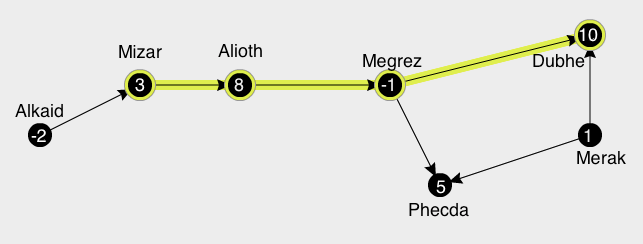
\includegraphics[max size={\textwidth}{\textheight}]{/Users/eevanikkari/PistepeliTira/dokumentaatioTexMuodossa//verkko1.PNG}

Paras reitti oli Mizar:3->Alioth:8->Megrez:-1->Dubhe:10, ja sen arvo oli 20.\\

\textbf{Verkko 2:}\\
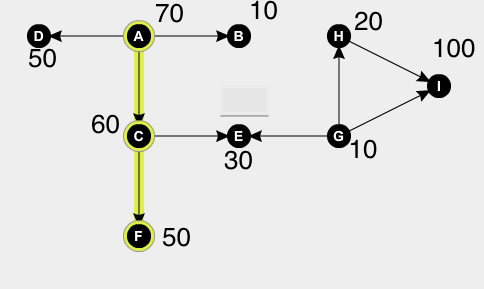
\includegraphics[max size={\textwidth}{\textheight}]{/Users/eevanikkari/PistepeliTira/dokumentaatioTexMuodossa//verkko2.PNG}

Paras reitti oli A:70->C:60->F:50, ja sen arvo oli 180.\\

\textbf{Verkko 3:}\\
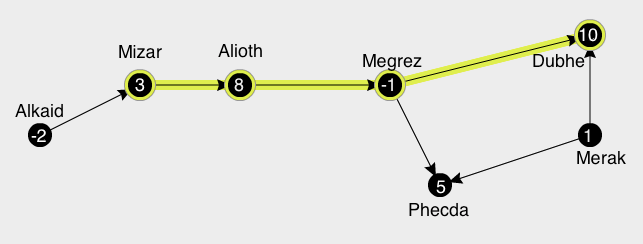
\includegraphics[max size={\textwidth}{\textheight}]{/Users/eevanikkari/PistepeliTira/dokumentaatioTexMuodossa//verkko3.PNG}

Paras reitti oli R:3->S:5->T:2->X:3->Y:4->Z:2, ja sen arvo oli 19.



Verkko 3 on sama verkko, kuin sivulla, jossa algoritmi on esitelty. Tässä tapauksessa, eli kun solmuilla on paino eikä kaarilla, se on kuitenkin jossain määrin triviaali, sillä algoritmi pääsee kulkemaan koko verkon läpi ja saa siis joka tapauksessa parhaan pistemäärän.
\\\\

\end{document}
 